

% Template PNSAC newsletter
% Language: Latex


\title{Canada Day 2016}
\author{Bill Tate}

\maketitle

Canada Day at the Museum always provides us with an opportunity to show off what
PNSAC is and does; and July 1, 2016 was no exception. Fortunately the weather
was ideal for most of the day. Our volunteers partially set up our display on
June 30th and the balance was done early in the morning of July1st.

Our display, unlike the picture shown below from 2011, was limited by the nose
section being shrink wrapped in plastic to prevent water damage. Consequently,
we unable to show off the cockpit because of lighting issues and ventilation.
This could have been rectified with additional fans and lights but with
restoration work being done on the main cabin floor, visits were limited to
viewing from just inside the aircraft rear cargo door.

Although not widely known we are also limited by the number of people. we can
have inside the aircraft at any one time. There is a reason for this as an empty
aircraft "generally" has the centre of gravity in the aft range limit and with
the engine \#4 off the aircraft this becomes even more pronounced. For this
reason sand bags have been placed in the forward cargo hold to help keep the
centre of gravity as far forward as possible. This limits us to having a maximum
of four adults or a family with children in at one time and yes we have to
include our volunteers so that we do not exceed the equivalent of six adults.


%\begin{figure}[htbp]
%   \vspace{2em}
%   \centering
%   %name of the graphic, without the path AND in EPS format:
%   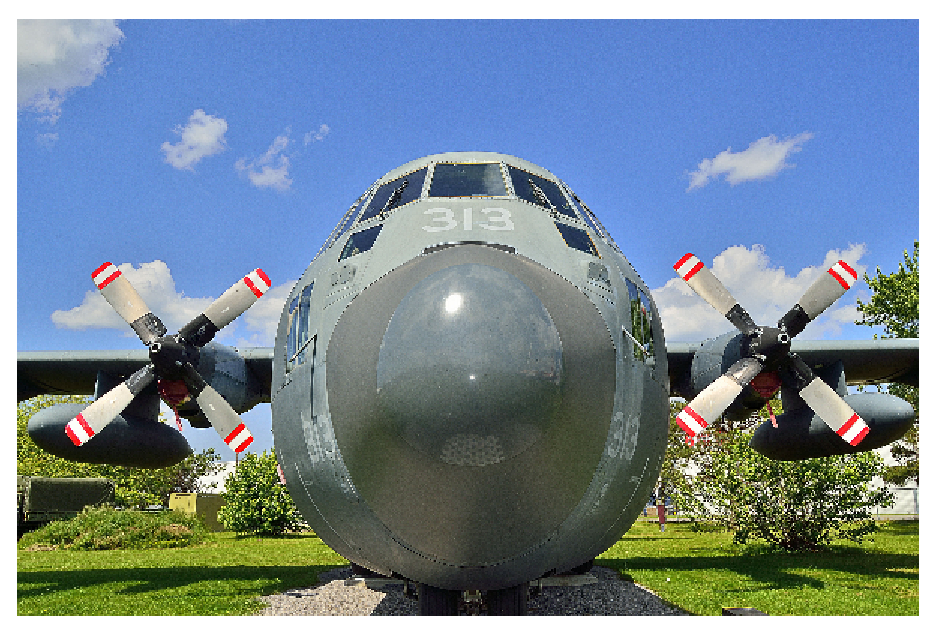
\includegraphics[scale=0.5]{trenton2013-herc.eps}
%   %caption of the figure 
%   \caption*{\small \em National Air Force Museum -- Hercules.}
%   %label of the figure, which has to correspond to \ref{}:
%   \label{fig:herc}
%\end{figure}


\end{multicols}

\begin{figure*}[ht!]
   \vspace{2em}
   \centering
   %name of the graphic, without the path AND in EPS format:
   \includegraphics[scale=0.75]{canada-day-2016}
   %caption of the figure 
   \caption*{\small \em Canada Day 2016.}
   %label of the figure, which has to correspond to \ref{}:
   \label{fig:canadaday}
\end{figure*}

\begin{multicols}{2}

The weather forecast that day was for thunder storm activity and as the day
progressed the skies darkened. For the safety of our volunteers and public we
shut down our display earlier than normal because as the wind increased we had
some of our story boards blown over by gusts of wind. As an aside, airports with
"Thor Guard" cease ramp operations when a thunderstorm is within 6 nautical
miles.

Our display attracted many visitors and there was a continuous line of people
waiting patiently for their turn to climb the steps and view the aircraft
interior. As in previous years we also took the covers off engine \#2 so we could
show an engine to our visitors after it had been fully restored.

I would like to thank all our volunteers who made Canada Day such a success and
to mention the very demanding work performed by Bruce Grant and Jim Riddoch who
handled crowd control, and John Thibert and Charles Baril who spent several
hours in the hot interior of the North Star talking to our visitors about the
work that went on inside the airplane.

Any suggestions to improve our display, who we are and what we do would be most
appreciated. Please send to Bill Tate.

\begin{footnotesize}
    \raggedleft PNSAC\\
\end{footnotesize}

%%% Local Variables: 
%%% mode: latex
%%% TeX-master: main_document.tex
%%% End: 
